Chương này trình bày chi tiết về đội hình đa robot, cấu trúc chữ V và việc thiết kế đường đi bao phủ cho đội hình chữ V đó để quét bao phủ môi trường cần khảo sát dạng đa giác lồi với mục tiêu tối ưu tỷ lệ bao phủ và tối thiểu thời gian di chuyển của đội hình.

\section{Kỹ thuật hình thành và duy trì đội hình đa robot, cấu trúc chữ V}
Phần này tập trung vào việc điều khiển các robot di chuyển trong một đội hình chữ V để quét một khu vực quan tâm, được gọi là khu vực khảo sát. Bầy robot sẽ có N con, trong đó mỗi robot sẽ được trang bị  các các cảm biến như là: cảm biến định vị GPS, cảm biến đo lường quán tính (IMU) để xác định vị trí và định hướng của nó đối với hệ tọa độ toàn cầu, một hệ thống cảm biến tránh va chạm để phát hiện trở ngại, một mô-đun mạng truyền thông không dây để thực hiện giao tiếp ngang hàng với các robot khác trong phạm vi của nó và cuối cùng là một máy ảnh để thực hiện khảo sát hình ảnh trên khu vực quan tâm. Tầm nhìn của máy ảnh (FOV) được xem là phạm vi bao phủ của một robot.

\subsection{Mô hình Leader-Follower}
Trong quá trình di chuyển theo đội hình, các robot sẽ được tổ chức theo mô hình leader-follower, trong đó mỗi thành viên đóng một vai trò như sau:
\begin{itemize}
    \item Leader: Robot dẫn đầu có nhiệm vụ di chuyển dọc theo đường đi được thiết kế trước và tạo ra cấu trúc ảo hình chữ V với đỉnh nằm ở vị trí của Robot đó. Các mục tiêu ảo trên cấu trúc ảo được chỉ định cho những người theo dõi thông qua mạng ad-hoc không dây.
        \item Follower: Robot theo sau thực hiện các nhiệm vụ tiếp nhận mục tiêu ảo được chỉ định, đồng thời di chuyển và theo dõi chặt chẽ mục tiêu của nó để tạo thành cấu trúc hình chữ V.
\end{itemize}

Trong quá trình bầy robot quét bao phủ, các Robot có nhiệm vụ duy trì đội hình chữ V đồng thời tránh va chạm với các chướng ngại vật và các Robot khác trong đội hình, bám đường đi bao phủ được thiết kế.

\subsection{Đội hình chữ V}
% {\color{red} formation dịch là đội hình, formation control dịch là điều khiển đổi hình => Rà soát để dùng thống nhất trong cả quyển. Mục này tên tiếng việt là Đội hình chữ V}
\label{sec:VTG}
\begin{figure}[hbtp]
    \centering
    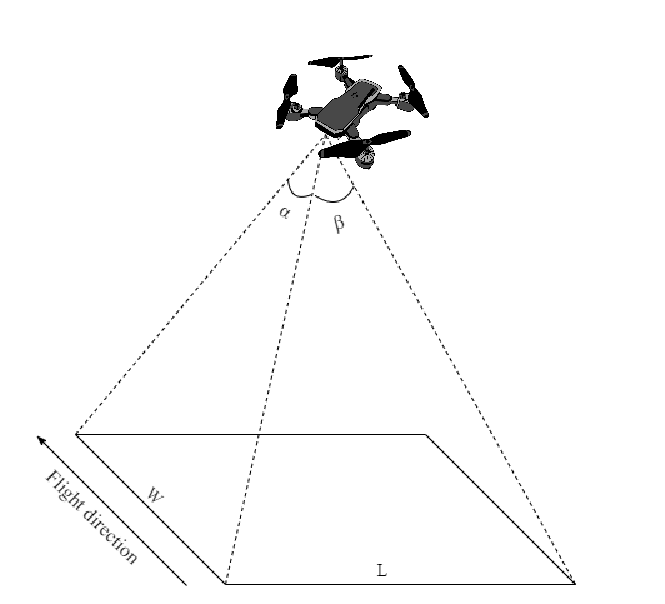
\includegraphics[width=0.5\textwidth]{chapter3/image/FOVDr.pdf}
    \caption{Camera's FOV}
    \label{fig:FOVmodel}
\end{figure}

Vùng bao phủ của mỗi Robot được xác định bởi phạm vi quan sát FOV (Field of View) của cảm biến chẳng hạn sử dụng camera có FOV như trong Hình \ref{fig:FOVmodel}. Với Robot có độ cao $h$, thì chiều rộng $W$ và chiều dài $L$ của FOV được xác định như sau:
\begin{equation}
    W = 2h\tan \frac{\alpha}{2}, \text{and }L = 2h \tan \frac{\beta}{2}
\label{eq:FOV}
\end{equation}
Trong đó $\alpha$ và $\beta$ lần lượt là độ dài theo phương dọc và ngang của camera

\begin{figure}[!t]
\centering
    \begin{subfigure}[b]{0.8\textwidth}
    \centering
    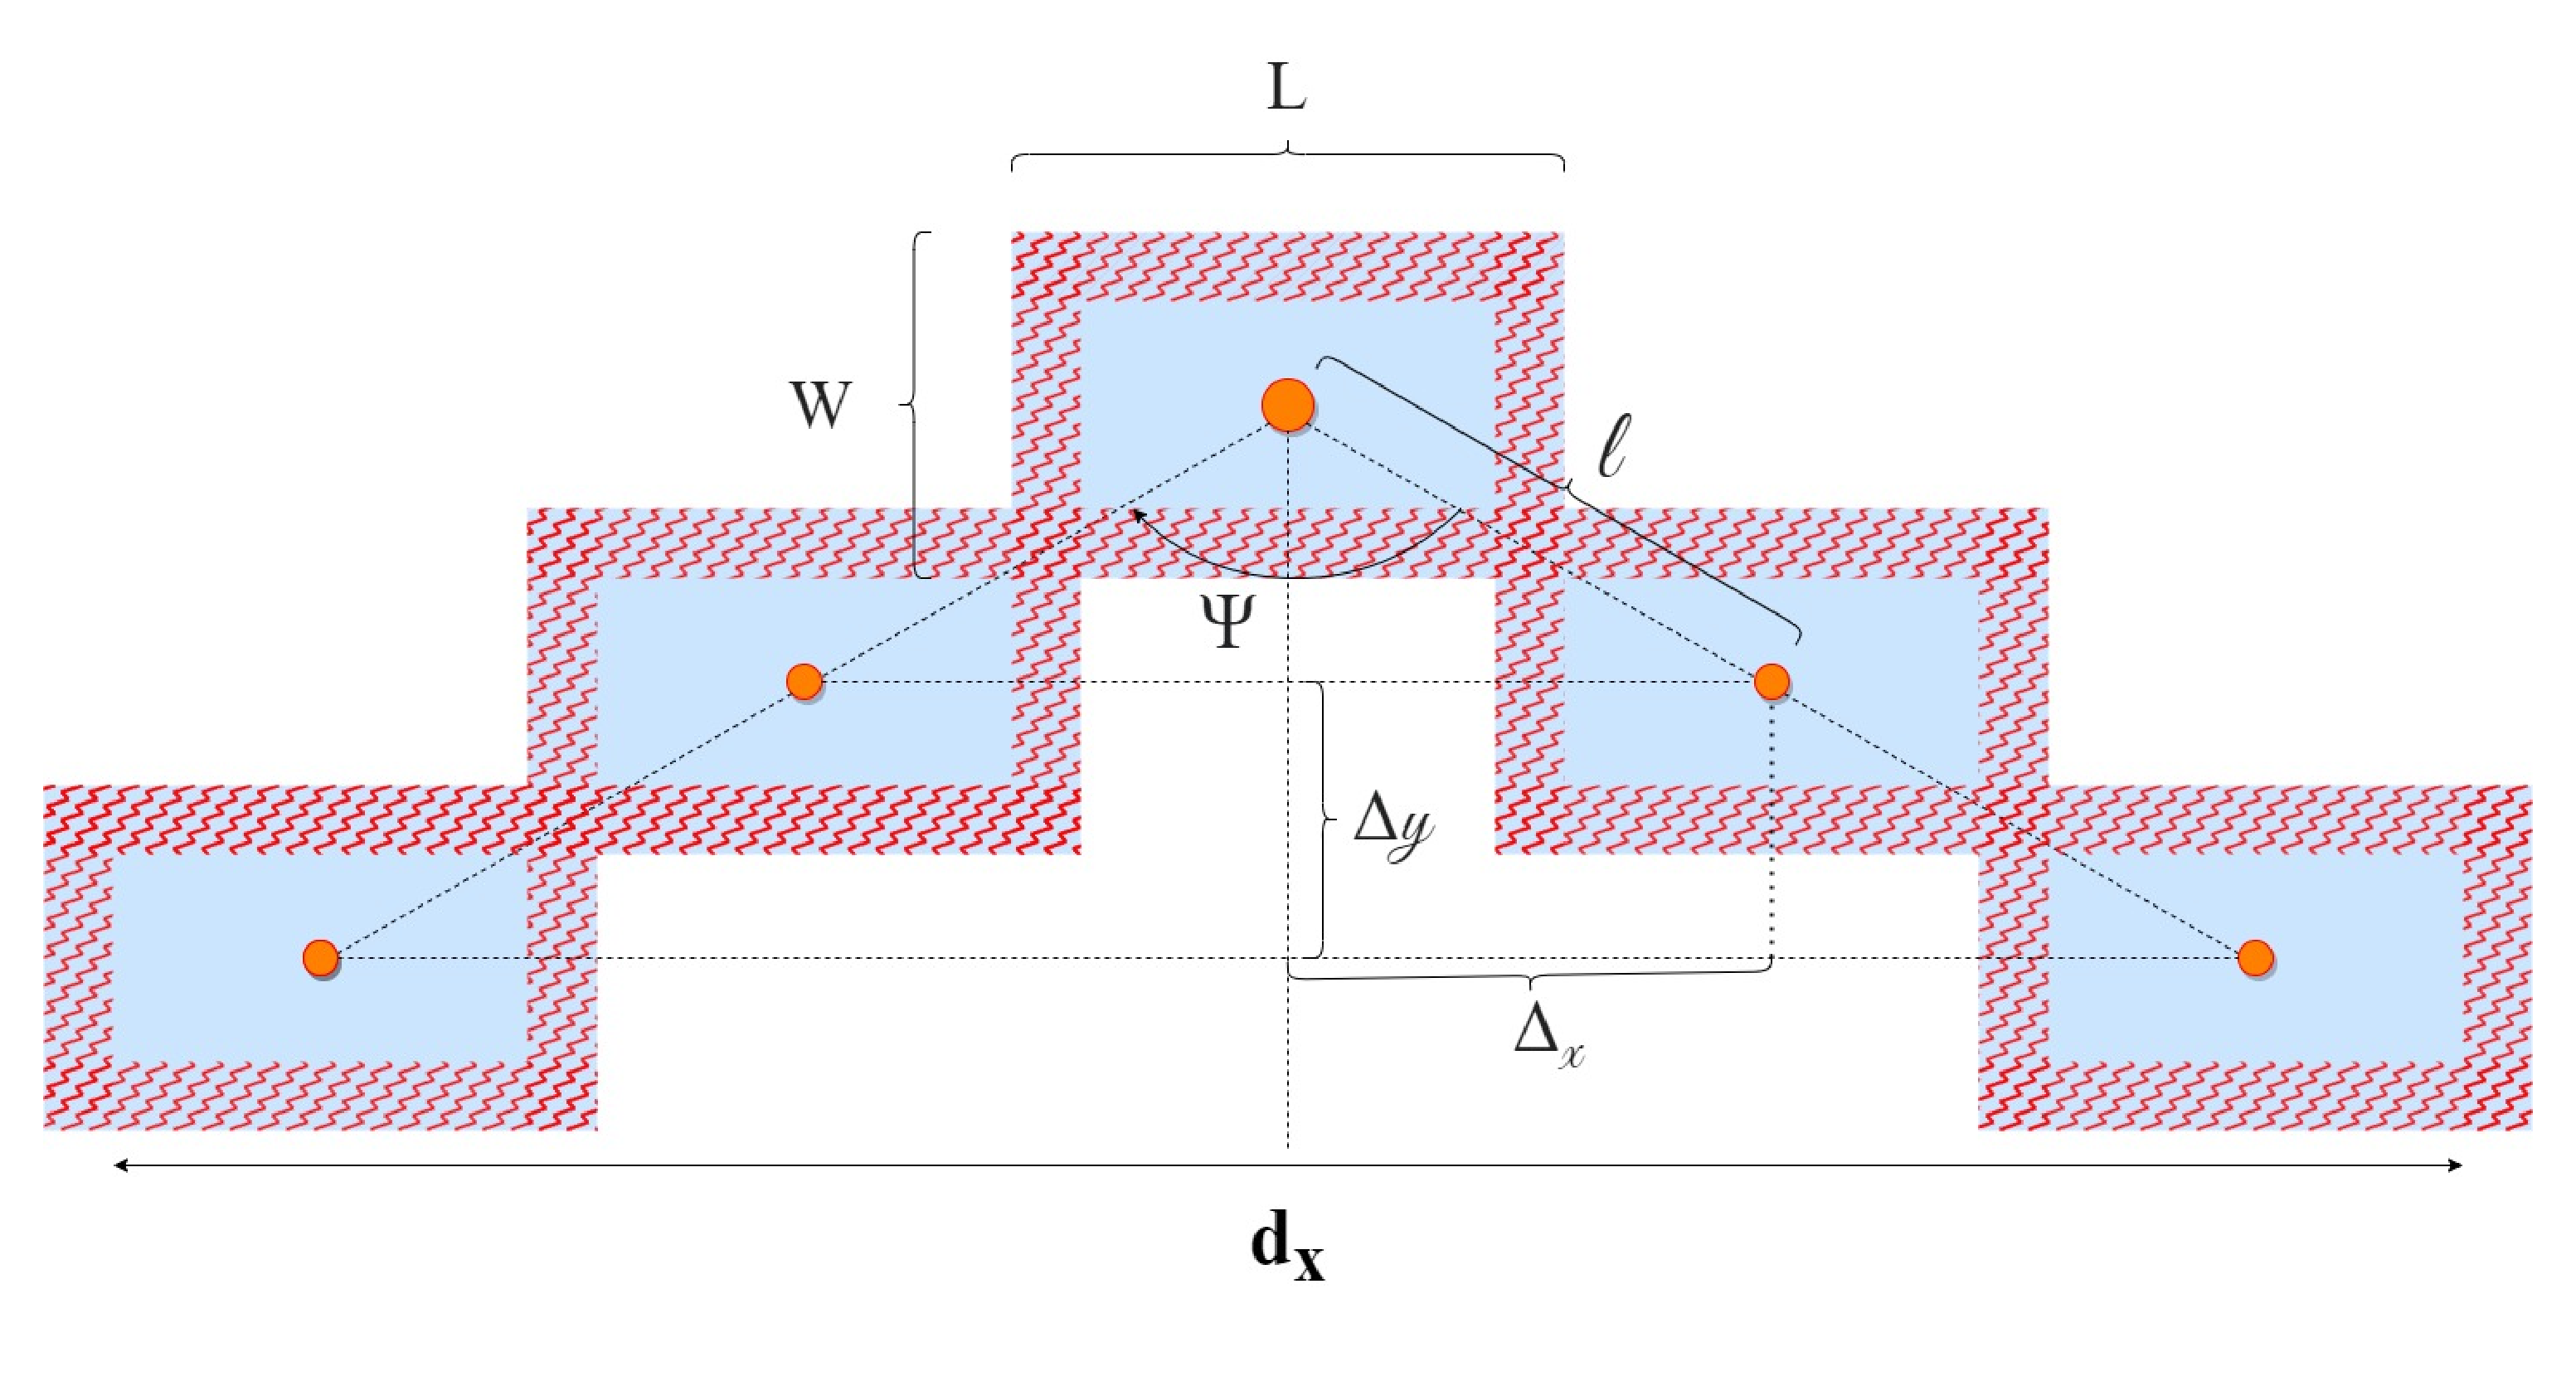
\includegraphics[width=\textwidth]{chapter3/image/SwarmRobotic_.drawio.pdf}
    \caption{Đội hình chữ V}
    \label{fig:Vshapemodel1}
    \end{subfigure}
    \begin{subfigure}[b]{0.6\textwidth}
    \centering
    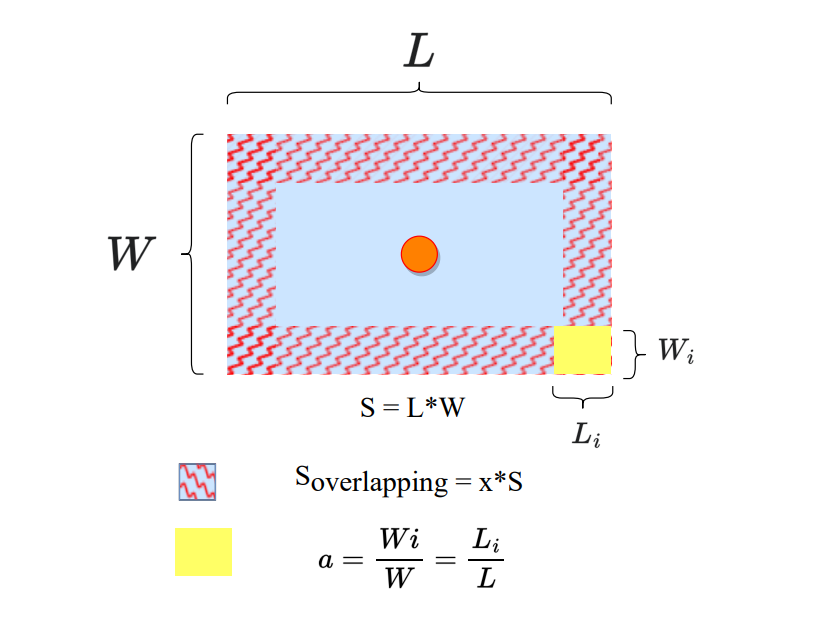
\includegraphics[width=\textwidth]{chapter3/image/a.png}
    \caption{Tỉ lệ trùng lặp của máy ảnh}
    \label{fig:Overlapingmodel1}
    \end{subfigure}
    \caption{Mô hình hệ thống cho việc hình thành nên đội hình chữ V}
    \label{fig:systemmodel}
%\vspace{-0.5cm}
\end{figure}

Đội hình chữ V của Robots được mô tả như Hình.\ref{fig:Vshapemodel1} tại đó $\psi$ là góc chữ V, và $\ell$ là khoảng cách tương đối giữa hai Robots liên tiếp trong đội hình. Tại thời điểm tùy ý, vùng bao phủ của bầy Robot được thể hiện bằng hình ảnh khảo sát được hợp nhất bởi các hình ảnh từ phạm vi quan sát FOV của tất cả các Robot. Quá trình ghép hình ảnh yêu cầu một tỷ lệ chồng chéo thích hợp $x$ $(0<x<1)$ để khắc phục sự biến dạng của ống kính và có đủ các tính năng có thể phát hiện được như được hiển thị trong Hình.\ref{fig:Overlapingmodel1}. Các tham số $\psi$ và $\ell$ của đội hình chữ V có thể dễ dàng xác định như sau: 
\begin{equation}
   S_{overlap}=2WLa+2(L-2La)Wx=4WLa-4WLa^{2}
\label{eq:S}
\end{equation}
 
Mặt khác $S_{overlap} = WLx$. Thay$S_{overlap}$ vào công thức \ref{eq:S} ta được :
\begin{equation}
\begin{array}{c}
   WLx=4WLa-4WLa^{2}\\
   \Rightarrow\dfrac{x}{4}=a-a^{2}
   \end{array}
\label{eq:PT3}
\end{equation}

Từ việc giải phương trình bậc 2, công thức \ref{eq:PT3} ta hoàn toàn có thể tìm ra giá trị a thỏa mãn. Từ đó suy ra $\l$ và $\psi$:
\begin{equation}
  \left\{ \begin{array}{c}
    \ell=\sqrt{\Delta_{x}^2+\Delta_{y}^2}\\
    \psi=2\text{atan2}(\Delta_{y},\Delta_{x})
    \end{array}\right.
\label{eq:PT4}
\end{equation}
Trong đó $\Delta_{x}=(1-a)L$ và $\Delta_{y}=(1-a)W$.\\

Leader sẽ tạo ra cấu trúc chữ V ảo trong hệ toạ độ toàn cầu mà trong đó đỉnh là vị trí của nó, các tham số $\psi_i$ và $\ell$ được xác định bởi công thức \ref{eq:PT4}. Qua đó, giả sử rằng $P_L=[x_L, y_L, z_L]^T$ và $\theta$ là vị trí của leader, và góc mục tiêu giữa véc tơ từ vị trí hiện tại của leader đối với mục tiêu và trục $x$ như trong Hình.\ref{fig:LF}. Đội hình chữ V có hai cánh trái và phải. được xác định lần lượt bởi góc quay $\varphi=\theta\mp\dfrac{\psi}{2}+\pi$. Các mục tiêu ảo được phân bổ đều cho hai bên cánh với khoảng cách $\ell$. Do đó, vị trí của các mục tiêu ảo được xác định dưới đây:
\begin{equation}
    P_T=Rot_z(\varphi)P_{t}+P_{L}
\end{equation}

\begin{equation}
   \begin{aligned}
       \left[\begin{array}{c}
       x_{T}\\
       y_{T}\\
       z_{T}
       \end{array}\right]=\left[\begin{array}{ccc}
       \cos\psi & -\sin\psi & 0\\
       \sin\psi & \cos\psi & 0\\
       0 & 0 & 1
       \end{array}\right] \left[\begin{array}{c}
       x_t\\
       y_t\\
       0
       \end{array}\right]
       +\left[\begin{array}{c}
       x_{L}\\
       y_{L}\\
       z_{L}
       \end{array}\right]
   \end{aligned}
   \label{eqn:method}
\end{equation}
Trong đó $Rot_z(\varphi)$ là ma trận xoay quanh trục z với góc quay $\varphi$; $P_t=[x_t, y_t,0]^T$ với $x_t=\pm i\l\cos\dfrac{\psi}{2}$, $y_t=\pm i\l\sin\dfrac{\psi}{2}$ lần lượt là vị trí của các mục tiêu ảo bên phải và trái đối với toạ độ địa phương của leader. Và $i=1,...,\left\lfloor\dfrac{(n-1)}{2}\right\rfloor $ thể hiện chỉ số của mục tiêu ảo của hai bên cánh.
\begin{figure}[h!]
    \centering
    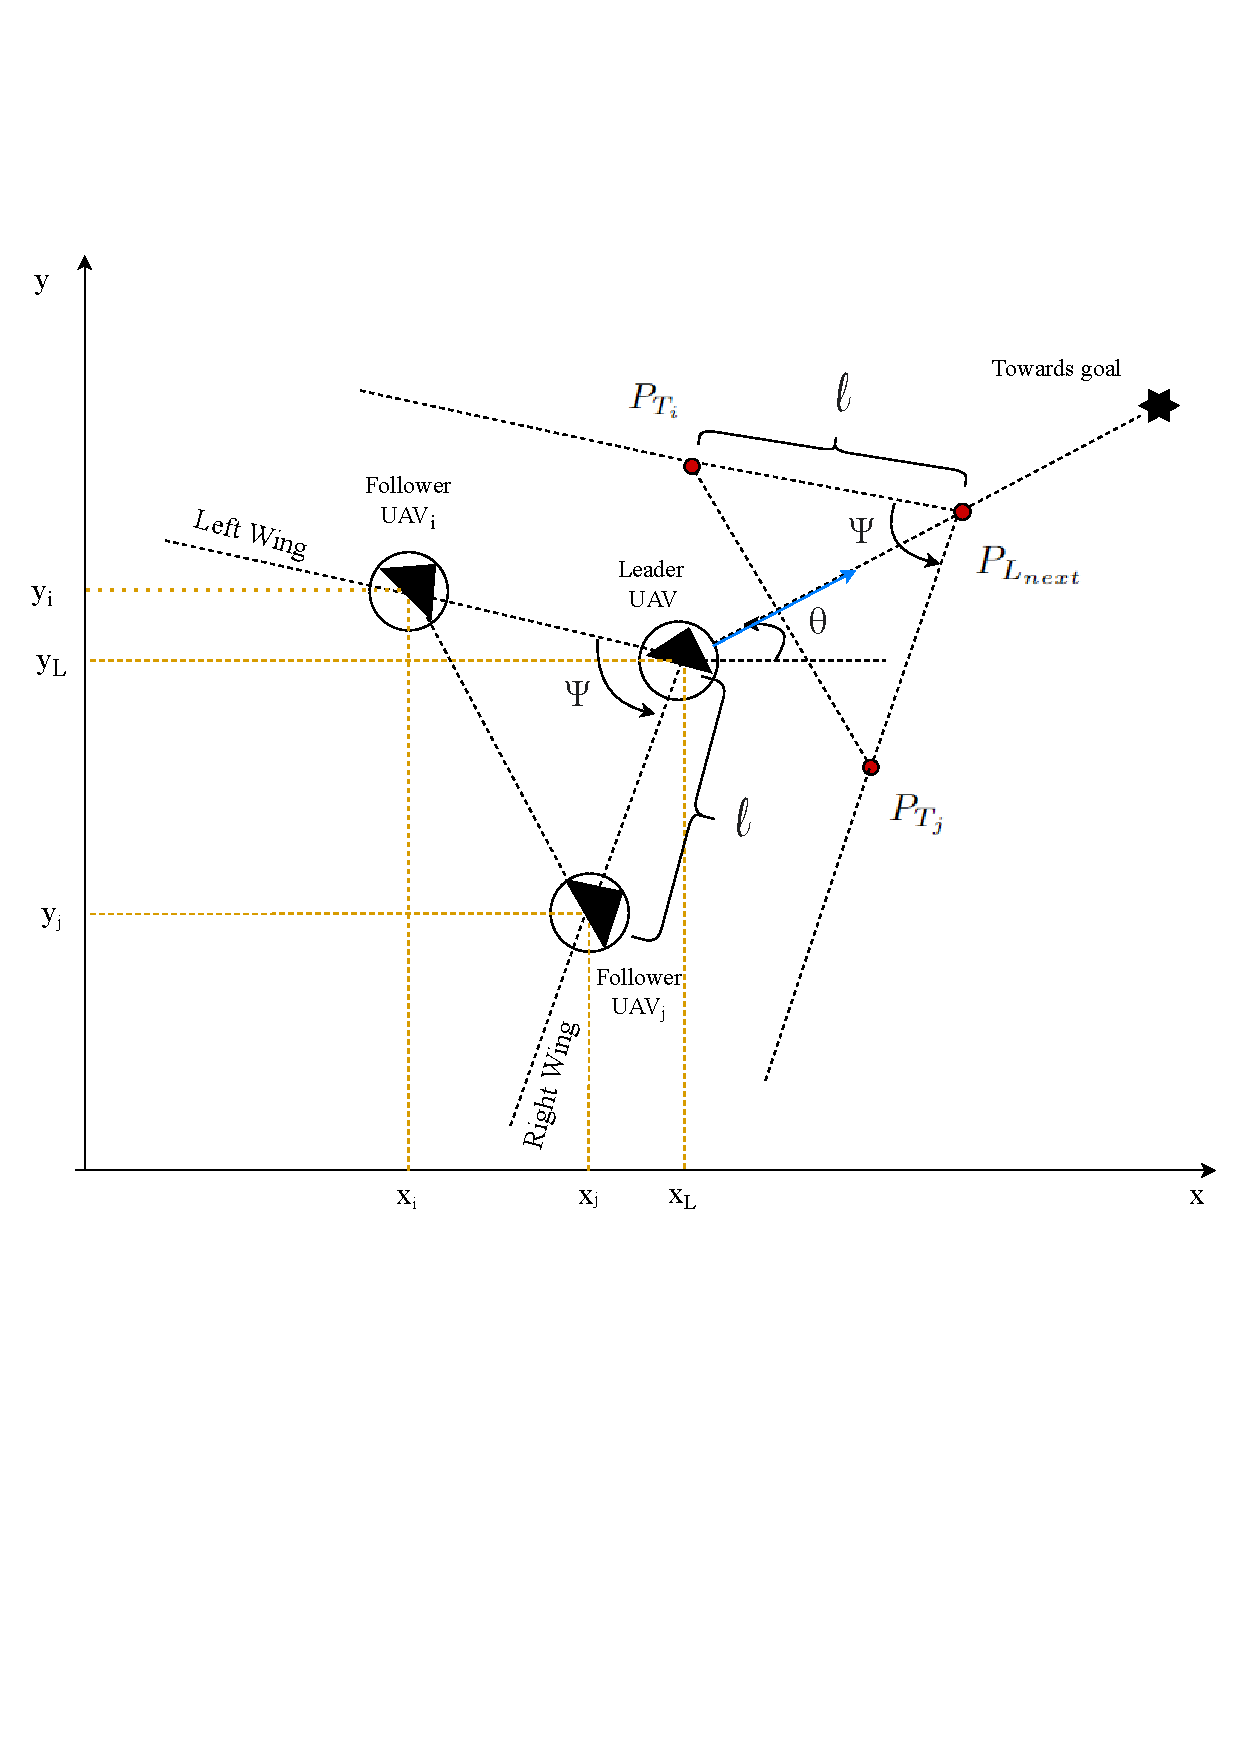
\includegraphics[width=0.7\textwidth]{chapter3/image/LF_Crop.pdf}
    \caption{Tạo cấu trúc chữ V ảo}
    \label{fig:LF}
\end{figure}
